\documentclass[11pt,a4paper, english, swedish
]{article}
\pdfoutput=1

\usepackage{custom_as}

\graphicspath{ {figurer/} }

%%Drar in tabell och figurtexter
\usepackage[margin=10 pt, size=small]{caption}
%%För att lägga in 'att göra'-noteringar i texten
\usepackage{todonotes} %\todo{...}

%%För att själv bestämma marginalerna. 
\usepackage[
%            top    = 3cm,
%            bottom = 3cm,
%            left   = 3cm, right  = 3cm
]{geometry}

%%För att ändra hur rubrikerna ska formateras
%\renewcommand{\thesection}{...}


\newcommand{\PP}[1]{\ensuremath\mathcal{P}\left(#1\right)}

\newcommand{\VAR}[1]{\ensuremath\text{var}\!\left[#1\right]}


%%%%%%%%%%%%%%%%%%%%%%%%%%%%%%%%%%%%%%%%%%%%%%%%%%%%%%%%%%%%%%%%%%%%%%
\newcounter{exempel_counter}%[section]
\newenvironment{exempel}
{
  \refstepcounter{exempel_counter}
  \begin{quote}
  \noindent\textbf{Exempel~\arabic{exempel_counter}:}
}{
  \end{quote}
}
%%%%%%%%%%%%%%%%%%%%%%%%%%%%%%%%%%%%%%%%%%%%%%%%%%%%%%%%%%%%%%%%%%%%%%

\begin{document}

%\newgeometry{top=1cm, bottom=2cm}
%%%%%%%%%%%%%%%%% vvv Inbyggd titelsida vvv %%%%%%%%%%%%%%%%%
\title{\huge Behandling av experimentella resultat\\[2mm] 
\Large En introduktion för fysikstudenter om hur man ska\\ hantera
mätresultat och feluppskattningar}
\author{
Andréas Sundström\footnote{
\href{mailto:sundstrom.andreas@gmail.com}{\nolinkurl{sundstrom.andreas@gmail.com}}
\: Jag tar gärna emot synpunkter och förslag.}
}
\date{\today, \quad\texttt{v\,0.1}}
\maketitle
%%%%%%%%%%%%%%%%% ^^^ Inbyggd titelsida ^^^ %%%%%%%%%%%%%%%%%



\noindent{\bf \large Förord}\\[1mm]
\small
Det här kompendiet är skrivet som en introduktion till
feluppskattningar för det svenska IPhO-laget. Jag har försökt fatta
mig kort, men jag har en tendens att kunna dra iväg när jag
skriver. Jag har försökt lägga innehållet på en nivå för att kunna
förstås av en gymnasieelev, men det är inte alltid det går så
bra\ldots{} Ni är de första som läser det här kompendiet. Tycker du
att det det här var för svårförståeligt så har \textbf{jag} skrivit
för komplicerat, och du är inte ensam om att tycka att kompediet var
svårt. \emph{Så säg till om det var krångligt!} 

\todo{Uppdatera }
Det viktigaste innehållet finns i avsnitt~\ref{sec:matfel},
men jag tyckte att det behövs en liten teoretisk bakgrund också, den
finns i avsnitt~\ref{sec:statistik}. Det avsnittet ska man läsa om man
vill få en lite klarare bild om varför feluppskattningarna beräknas på
det ena eller andra viset. Avslutningsvis räknas ett exempel med lite
olika feluppskattningar.

Sedan har jag även lagt till en bilaga om
Taylorutvecklingar. Den hör inte så mycket ihop med resten av det här
kompendiet, men det är matnyttigt att kunna göra uppskattningar både
för teoretiska och experimentella beräkningar.  

\begin{flushright}
Andréas Sunsdtröm\\ 
Göteborg, 2016-06-12
\end{flushright}
\normalsize



\clearpage
\tableofcontents
\clearpage

%\restoregeometry

\setcounter{page}{1}
%\addtocounter{section}{-1}



\setcounter{section}{-1}
\section{Sannolihetslära och statistik (överkurs)}\label{sec:statistik}
När man gör mätningar vill man oftast ta reda på någon storhets värde
-- exempelvis periodtiden på en pendel. Med en mätning kan man dock
inte säga något om hur bra mätningen var. Men med flera mätningar kan
vi börja göra statistik över dem. Då 

Jag vill även betona vikten av statistik i framtida vetenskapliga och
tekniska karriärer. \emph{Statistik är ett mycket kraftfullt verktyg.}
Statistiken, när man börjar behärska den, är mycket mer än bara
''medelvärden och standardavvikelser''; den spelar en väsentlig roll i
mer eller mindre all experimentell vetenskap -- särskilt vid
feluppskattningar. 

\subsection{Stokastiska variabler}
Precis som vanliga variabler används stokastiska variabler för att
beteckna något okänt. Men i fallet med stokastiska variabler saknar de
ett värde. De är mer tänkta som ett koncept för att betecka en
slumpartad händese eller process. Man kan gör en observation/mätning
av en stokastisk variabel och få ett värde, men det är bara ett
mätvärde som man kan få. 

\begin{exempel}
Ett tärningskast är ett exempel som kan beskrivas med en diskret
stokastisk variabel. Låt den stokastiska variabeln $X$ beskriva
tärningskastet. Den kan då mätas till ett visst utfall 
$x$. I fallet med en tärning $X$ har ett utfallsrum som består av
talen 1 till 6: $\{1, 2, 3, 4, 5, 6\}$. Varje element i utfallsrummet
har också en viss sannolikhet, $\nicefrac{1}{6}$ i det här fallet.
 
Själva variablen $X$ (tärningen) kan alltså inte i sig ha ett värde.
Men när man gör en observation (kastar tärningen) kan man få ett
mätresultat $x$, som (när tärningen är kastad) har ett fast värde.
\end{exempel}

Fördelen med att ha stokastiska variabler är att man, likt vanliga
variabler, kan börja räkna med dem mer generellt än om man bara har
vissa specialfall. I det här kompendiet kommer de att användas, men
inte med så stor vikt. (Stokastiska variabler kommer här att betecknas
med stora bokstäver.)

\subsection{Sannolikhetsfördelningar och täthetsfunktioner}
Den statistik och sannolikhetslära man får lära sig i gymnasiet brukar
fördet mesta vara diskret (och ändlig). Alltså att det finns ett
ändligt antal möjliga utfall och varje utfall är distikt. Exempel på
detta är tärningskast, lottdragning och kortlekar. 

Verkligheten är dock oftast mer komplicerad än så. När man gör
mätningar handrar det oftas om mätnigar av en reellvärd
storhet som t.ex. en längd\footnotemark{}. Detta betyder att längden
kommer att anta ett reellt antal milimetrar och inte vara begränsad
till ett ändligt antal möjliga värden. För att analysera detta behövs
statistik för kontinuerliga fördelningar. 
\footnotetext{''Aha!'' tänker ni: atomer och kvantfysik gör att det
  bara finns diskreta längder. ''Nähä!'' säger jag: som fysiker måste
  man kunna hantera approximationer och veta begränsningarna i sina
  mätningar. Med en linjal eller skujtmått finns det ingen chans i
  världen att man skulle kunna stöta på problem orsakade av
  kvantfysik. Man kan alltså betrakta det som om de möjliga värden
  som längden kan anta ligger kontinuerligt.}

Sannolikhetsfördelningar karakteriseras av sin täthetsfunktion, som
brukar betecknas~$f$. Täthetsfunktionen talar om hur sannolikt det är
att få ett värde i ett visst intervall. Notera dock att den
\emph{inte} ger sannolikheten att få ett specifikt värde. 
Eftersom det finns (ouppräknerligt) oändligt många möjliga utfall så
är sannolikheten att få ett visst exat värde
\begin{equation}
\PP{X=x}\; \text{''=''}\; \frac{1}{\infty}\; \text{''=''}\;0.
\end{equation}
För att istället beräkna sannolikheten att få sitt utfall $X$ i ett
visst intervall $[a, b]$ måste man integrera:
\begin{equation}\label{eq:dist_P}
\PP{a<X<b} = \int_a^b f(x) \id{x}.
\end{equation}
Sannolikheten att få $a<X<b$ bestäms alltså av arean under $f(x)$.

\begin{exempel}
Sannolikheten för en radioaktiv kärna att sönderfalla kan beskrivas
med den så kallade exponentialfördelningen:
\begin{equation*}
f(t)=
\begin{cases}
\lambda\ee^{-\lambda t},& t>0\\
0 ,& t\le0,
\end{cases}
\end{equation*}
där $\lambda$ är en konstant som kallas isotopens
sönderfallskonstant. 
Vad är sannolikheten att kärnan har sönderfallit vid tiden
$\tau=\nicefrac{\ln(2)}{\lambda}$? 

Sannolikheten att en kärna sönderfaller mellan tiden $0$ och $\tau$
ges enligt \eqref{eq:dist_P} helt enkelt av integralen
\begin{equation*}
\PP{0<T_\text{sönderfall}<\tau} 
= \int_0^\tau\lambda\ee^{-\lambda t}\id{t} 
= \lambda\,\frac{\ee^{0}-\ee^{-\lambda \tau}}{\lambda}
= 1-\ee^{-\lambda \tau}
=1-\frac{1}{2} = \frac{1}{2}.
\end{equation*}
Tiden $\nicefrac{\ln(2)}{\lambda}$ är alltså isotopens halveringstid. 
\end{exempel}



\subsubsection{Normalfördelningen}
En av de vanligaste fördelningarna är normalfördelningen. Den
har täthesfunktionen
\begin{equation}
f(x) = \frac{1}{\sqrt{2\pi\sigma^2}} \, \ee^{-\frac{(x-\mu)^2}{2\sigma^2}},
\end{equation}
där $\mu$ är fördelningens \emph{väntevärde} och $\sigma$ är dess
\emph{standardavvikelse}. I \figref{fig:normal_dist} visas
täthetsfunktionen för några olika val av $\mu$ och $\sigma$. Där ser
vi att $\mu$ svarar mot var någonstans fördelnigen är centrerad, och
att $\sigma$ svarar mot hur bred fördelningen blir. 

Som kan ses i \figref{fig:normal_dist} går sannolikhetsfördelningen
ner och blir väldigt liten för värden långt ifrån $\mu$. Till exempel
ligger ca 98\,\% av all sannolikhet/area under kurvan inom $\mu\pm
2\sigma$, men sen går det snabbt -- fortsätter man uppåt så ligger
99,99997\,\% inom $\mu\pm 5\sigma$.

\begin{figure}
\centering
% GNUPLOT: LaTeX picture with Postscript
\begingroup
  \makeatletter
  \providecommand\color[2][]{%
    \GenericError{(gnuplot) \space\space\space\@spaces}{%
      Package color not loaded in conjunction with
      terminal option `colourtext'%
    }{See the gnuplot documentation for explanation.%
    }{Either use 'blacktext' in gnuplot or load the package
      color.sty in LaTeX.}%
    \renewcommand\color[2][]{}%
  }%
  \providecommand\includegraphics[2][]{%
    \GenericError{(gnuplot) \space\space\space\@spaces}{%
      Package graphicx or graphics not loaded%
    }{See the gnuplot documentation for explanation.%
    }{The gnuplot epslatex terminal needs graphicx.sty or graphics.sty.}%
    \renewcommand\includegraphics[2][]{}%
  }%
  \providecommand\rotatebox[2]{#2}%
  \@ifundefined{ifGPcolor}{%
    \newif\ifGPcolor
    \GPcolortrue
  }{}%
  \@ifundefined{ifGPblacktext}{%
    \newif\ifGPblacktext
    \GPblacktexttrue
  }{}%
  % define a \g@addto@macro without @ in the name:
  \let\gplgaddtomacro\g@addto@macro
  % define empty templates for all commands taking text:
  \gdef\gplbacktext{}%
  \gdef\gplfronttext{}%
  \makeatother
  \ifGPblacktext
    % no textcolor at all
    \def\colorrgb#1{}%
    \def\colorgray#1{}%
  \else
    % gray or color?
    \ifGPcolor
      \def\colorrgb#1{\color[rgb]{#1}}%
      \def\colorgray#1{\color[gray]{#1}}%
      \expandafter\def\csname LTw\endcsname{\color{white}}%
      \expandafter\def\csname LTb\endcsname{\color{black}}%
      \expandafter\def\csname LTa\endcsname{\color{black}}%
      \expandafter\def\csname LT0\endcsname{\color[rgb]{1,0,0}}%
      \expandafter\def\csname LT1\endcsname{\color[rgb]{0,1,0}}%
      \expandafter\def\csname LT2\endcsname{\color[rgb]{0,0,1}}%
      \expandafter\def\csname LT3\endcsname{\color[rgb]{1,0,1}}%
      \expandafter\def\csname LT4\endcsname{\color[rgb]{0,1,1}}%
      \expandafter\def\csname LT5\endcsname{\color[rgb]{1,1,0}}%
      \expandafter\def\csname LT6\endcsname{\color[rgb]{0,0,0}}%
      \expandafter\def\csname LT7\endcsname{\color[rgb]{1,0.3,0}}%
      \expandafter\def\csname LT8\endcsname{\color[rgb]{0.5,0.5,0.5}}%
    \else
      % gray
      \def\colorrgb#1{\color{black}}%
      \def\colorgray#1{\color[gray]{#1}}%
      \expandafter\def\csname LTw\endcsname{\color{white}}%
      \expandafter\def\csname LTb\endcsname{\color{black}}%
      \expandafter\def\csname LTa\endcsname{\color{black}}%
      \expandafter\def\csname LT0\endcsname{\color{black}}%
      \expandafter\def\csname LT1\endcsname{\color{black}}%
      \expandafter\def\csname LT2\endcsname{\color{black}}%
      \expandafter\def\csname LT3\endcsname{\color{black}}%
      \expandafter\def\csname LT4\endcsname{\color{black}}%
      \expandafter\def\csname LT5\endcsname{\color{black}}%
      \expandafter\def\csname LT6\endcsname{\color{black}}%
      \expandafter\def\csname LT7\endcsname{\color{black}}%
      \expandafter\def\csname LT8\endcsname{\color{black}}%
    \fi
  \fi
  \setlength{\unitlength}{0.0500bp}%
  \begin{picture}(6802.00,3968.00)%
    \gplgaddtomacro\gplbacktext{%
      \csname LTb\endcsname%
      \put(946,704){\makebox(0,0)[r]{\strut{} 0}}%
      \csname LTb\endcsname%
      \put(946,1454){\makebox(0,0)[r]{\strut{} 0.1}}%
      \csname LTb\endcsname%
      \put(946,2204){\makebox(0,0)[r]{\strut{} 0.2}}%
      \csname LTb\endcsname%
      \put(946,2953){\makebox(0,0)[r]{\strut{} 0.3}}%
      \csname LTb\endcsname%
      \put(946,3703){\makebox(0,0)[r]{\strut{} 0.4}}%
      \csname LTb\endcsname%
      \put(1078,484){\makebox(0,0){\strut{}-6}}%
      \csname LTb\endcsname%
      \put(1966,484){\makebox(0,0){\strut{}-4}}%
      \csname LTb\endcsname%
      \put(2854,484){\makebox(0,0){\strut{}-2}}%
      \csname LTb\endcsname%
      \put(3742,484){\makebox(0,0){\strut{} 0}}%
      \csname LTb\endcsname%
      \put(4629,484){\makebox(0,0){\strut{} 2}}%
      \csname LTb\endcsname%
      \put(5517,484){\makebox(0,0){\strut{} 4}}%
      \csname LTb\endcsname%
      \put(6405,484){\makebox(0,0){\strut{} 6}}%
      \put(176,2203){\rotatebox{-270}{\makebox(0,0){\strut{}$f(x)$}}}%
      \put(3741,154){\makebox(0,0){\strut{}$x$}}%
    }%
    \gplgaddtomacro\gplfronttext{%
      \csname LTb\endcsname%
      \put(2530,3475){\makebox(0,0)[r]{\strut{}$\mu=0$, $\sigma=1$}}%
      \csname LTb\endcsname%
      \put(2530,3255){\makebox(0,0)[r]{\strut{}$\mu=0$, $\sigma=2$}}%
      \csname LTb\endcsname%
      \put(2530,3035){\makebox(0,0)[r]{\strut{}$\mu=2$, $\sigma=1$}}%
    }%
    \gplbacktext
    \put(0,0){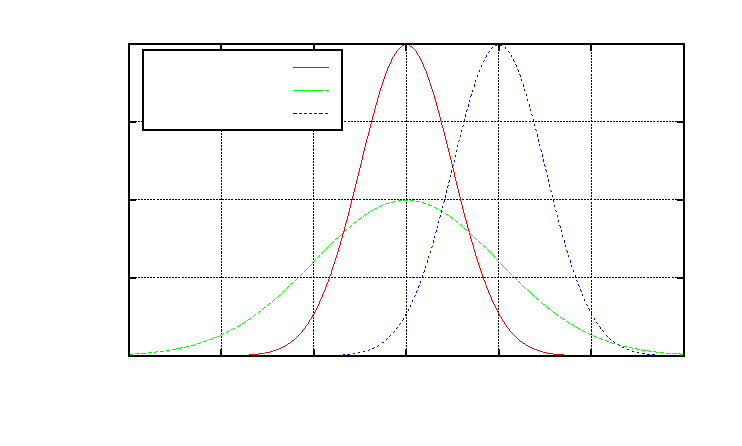
\includegraphics{normal_dist}}%
    \gplfronttext
  \end{picture}%
\endgroup

\caption{Täthetsfunktioner till normalfördelningar med olika värden på
väntevärdet $\mu$ och standardavvikelsen $\sigma$. Varje kurva har den
klassiska Gau\ss{}iska klockformen.}\label{fig:normal_dist}
\end{figure}

Kvadraten i exponentialen ger täthetsfunktionen den
klassiska klockformen hos en Gau\ss{}isk kurva, och faktorn framför
säkerställer att den totala integralen
\begin{equation}
\int_{-\infty}^{\infty} f(x)\id{x} = 1.
\end{equation}
Detta är något som \emph{gäller för alla täthetsfunktioner}. 


Normalfördelningen kallas just ''normal'' för att det finns en sats
som säger att i princip alla slumpfenomen blir normalfördelade om
samma process upprepas väldigt många gånger. Ett exempel på detta är
om man sannolikheten att få ett visst antal ''klave'' efter flera
slantsinglingar. Den här egenskapen gör att de allra flesta 
\emph{mätfelen antas vara normalfördelade}.

% Vidare är normalfördelningen en väldigt trevlig fördelning att arbeta
% med. Regeln för normalfördelningar är att om $X$ och $Y$ båda är
% normalfördelade och oberoende med väntevärde $\mu_X$ och
% standardavvikelse $\sigma_X$ respektive $\mu_Y$ och $\sigma_Y$, så är 
% \begin{equation}
% Z=\alpha X + \beta Y
% \end{equation}
% också normalfördelad med väntevärde $(\alpha\mu_X+\beta\mu_Y)$ och
% standardavvikelse $\sqrt{\alpha^2\sigma_X^2 + \beta^2\sigma_Y^2}$. 
% Med andra ord funkar väntevärdena som man kan tro och
% standardavvikelserna fungerar lite som Pythagoras sats. 


\subsection{Väntevärden, varianser och standradavvikelser}
De vanligaste fördelningarna har, som normalfördelningen, väntevärde
och varians. Dessa beräknas med täthetsfunktionen. Det är också dessa
som främst används i felanalys.

Väntevärdet av den stokastiska ariabeln $X$, med täthetsfunktion $f$,
definieras som 
\begin{equation}\label{eq:ev}
\ev{X} = \mu = \int_{-\infty}^\infty x f(x)\id{x}.
\end{equation}
Det är inte helt kart vad tolkningen ska vara direkt från
definitionen, men man kan jämföra väntevärdesintegralen med en slags
tyngdpunktsberäkning. Man lägger ihop varje punkts
''sannolikhetsmassa'', $f(x)\dd{x}$, gånger punktes avstånd, $x$, från
origo; till slut får man den sammanlagda tyngdpunkten. Man kan
faktiskt hitta en fördelnings väntevärde genom att kippa ut en (styv)
pappersbit formad efter ytan under kurvan och balanseta den utklippta formen. 

Sedan kan variansen definieras med hjälp av väntevärden:
\begin{equation}\label{eq:var}
\VAR{X} = \sigma^2 =\ev{(X-\mu)^2}. %\ev{X^2} - \mu^2.
\end{equation}
%Det sista ledet ovan är ett sätt som man kan skriva om variansen, men
%det används mest i teoretiska analyser och är inte så viktigt i
%nuläget. 
Tolkningen av variansen är att det är ett väntevärde på hur
mycket avvikelse man får från $\mu$, men för att ta med både positiva
och negativa avvikelser kvadreras de innan man tar väntevärdet.
Härifrån syns också att \emph{standardavvikelsen ges som roten ur
variansen}. 

\subsubsection{Några nyttiga satser}\label{sec:satser}
Det viktigaste man behöver veta om väntevärden är att de är
linjära. Alltså att
\begin{equation}\label{eq:ev_lin}
\Big\langle \alpha X + \beta Y + \gamma \Big\rangle 
= \alpha\ev{X} + \beta\ev{Y} + \gamma,
\end{equation}
för godtyckliga stokastiska variabler $X$ och $Y$ samt några
konstanter $\alpha$, $\beta$ och $\gamma$. Den här regen kan utvidgas
till ett godtyckligt antal variabler. 

För variansen gäller en liknande regel 
\begin{equation}\label{eq:var_lin}
\text{var}\!\Big[ \alpha X + \beta Y + \gamma \Big] 
= \alpha^2\VAR{X} + \beta^2\VAR{Y}, 
\end{equation}
men här måste $X$ och $Y$ vara statistiskt
oberoende\footnotemark{}. Även här kan man utvidga regeln till ett
godtyckligt antal oberoende variabler.
\footnotetext{Statistiskt oberoende är en ganska knepig term att
  deffiniera. Men enkelt sett så betyder det ungefär vad magkänslan
  säger: att resultatet av en mätning på den ena ska inte påverka
  resultatet på den andra. }

Speciellt gäller att om man har $N$ stycken oberoende stokastiska variabler
$X_i$ med lika fördelning och man vill ta ett medelvärde 
\begin{equation} 
\bar{X} = \frac{X_1+X_2+\cdots+X_N}{N} = \frac{1}{N}\sum_{i=1}^N X_i
\end{equation}
så kan man beräkna dess väntevärde och varians med hjälp av reglerna
ovan. 
Väntevärdet ges då från \eqref{eq:ev_lin} som
\begin{equation}\label{eq:ev_mean}
\ev{\bar{X}} = \ev{\frac{1}{N} \sum_{i=1}^N X_i} 
= \frac{1}{N} \sum_{i=1}^N \overbrace{\ev{X_i}}^{=\mu} 
= \mu,
\end{equation}
där $\mu$ är väntevärdet av varje enskild variabel från den givna
fördelningen. 
Variansen får man med \eqref{eq:var_lin} sedan som
\begin{equation}\label{eq:var_mean}
\VAR{\bar{X}} = \VAR{\frac{1}{N} \sum_{i=1}^N X_i}
= \VAR{\sum_{i=1}^N \frac{1}{N} X_i}
= \sum_{i=1}^N \frac{1}{N^2}\overbrace{\VAR{X_i}}^{=\sigma^2}
= \frac{\sigma^2}{N}.
\end{equation}
Dessa resultat kommer att användas i feluppsattningar genom att
betrakta varje mätning som en obervarion av respektive $X_i$.

\subsubsection{Skattning från mätdata}
Har man ett stokastiskt system och vill försöka mäta dess väntevärde
och standardavvikelse, så måste man ha många mätningar på det. Det är
nu som statistiken kommer in i bilden -- hur man behandlar tagna
mätningar av en stokastisk variabel. 

Från \eqref{eq:ev_mean} visade det sig att väntevärdet av ett
medelvärde är samma som väntevärdet av det man mäter på. Vidare visade
det sig att variansen av medelvärdet minskade som
$\nicefrac{1}{N}$. Tillsammans ger detta att \emph{ju fler mätningar
  man gör desto större är sannolikheten att medelvärdet man får blir
  just väntevärdet}. Detta betyder att man kan skatta väntevärdet med
\begin{equation}\label{eq:ev_approx}
\ev{X} = \mu \approx \bar{x} = \frac{1}{N}\sum_{i=1}^N x_i.
\end{equation}
Här användes små bokstäver $x_i$ för att beteckna att de är tagna
mätvärden -- de har alltså ett fast värde. 

Om nu väntevärden gick att skatta som medelvärden bör man väl kunna
göra det samma för varianser. Definitionen av varians i \eqref{eq:var}
består ju av två väntevärden (två stycken eftersom $\mu=\ev{X}$), så
det borde gå att skatta variansen med medelvärdet av
$(x_i-\bar{x})^2$. Svaret är att det  nästan går. Eftersom man bara
får ett ungefärligt värde på $\mu$ från \eqref{eq:ev_approx} måste
medelvärdet justeras något. Det visar sig att man ska använda
\begin{equation}\label{eq:var_approx}
\VAR{X} = \sigma^2 \approx s^2 = \frac{1}{N-1}\sum_{i=1}^N (x_i-\bar{x})^2
\end{equation}
för att skatta variansen. Standardavvikelsen fås enkelt genom att dra
roten ur skattningen av variansen:
\begin{equation}\label{eq:std_approx}
\sigma \approx s = \sqrt{\frac{1}{N-1}\sum_{i=1}^N (x_i-\bar{x})^2}.
\end{equation}
Detta kallas \emph{standradfelet} och är det namn som man har gett
till skattningen av standardavvikelsen.
Notera att $s$ är standradfelet i uppsättnigen av alla
mätpunkter. För att få \emph{standardfelet i medelvärdet}
använder man \eqref{eq:var_mean} och får $\nicefrac{s}{\sqrt{N}}$.




\section{Olika typer av mätfel}\label{sec:matfel}
När man vill uppskatta hur stora experimentella fel/osäkerheter man
har finns det två typer av fel och två typer av feluppskattningar. De
två typerna av fel som finns är systematiska och statistiska. Sedan är
de två typerna av feluppskattningar som man behöver kunna. Dels direkt
feluppskattning (av statistiska fel), dels propagering av osäkerhet. 


\subsection{Systematiska fel -- noggrannhet och precision}
\begin{figure}
\centering
\resizebox{0.5\textwidth}{!}{
\input{figurer/precision_noggrannhet.pdf_t}
}
\caption{Illustration av skillnaden mellan noggrannhet och
  precision. Måltavlorna representerar en mätning, där mitten på
  måltavlan svarar mot det ''sanna'' värdet. Fallen med låg
  noggrannhet svarar mot systematiska fel som inte går att avhjälpa
  med medelvärden av fler mätningar.}
\label{fig:prec_nog}
\end{figure}

Ett systematiskt fel är något som gör att ens mätresultat hela tiden
är lite fel åt något håll\footnotemark{}. Dessa karakteriseras av att
det inte hälper med flera mätningar för att få bättre mätresultat.
\footnotetext{Det behöver inte nödvändigtvis vara så att det är just
  fel åt samma håll hela tiden, men oftast är ett systematiskt fel
  något som ger en förskjutning av ens mätresultat.}

Man brukar skilja på två olika typer av godhet i mätningar. Det finns
dels noggrannhet, dels precision. Noggrannhet, eller rikighet som det
ibland kallas, svarar mot hur nära det ''sanna''\footnotemark{} värdet
mätningarna kommer i medel. Prescisionen svarar å andra sida mot hur
tätt mätresultaten hamnar, eller hur liten spridning man får i dem. De
två koncepten illustreras i \figref{fig:prec_nog}.  
\footnotetext{Jag sätter ''sanna'' inom citationstecken för att ur ett
experimentalistiskt perspektiv finns det inget sätt att veta det
verkligt sanna värdet -- man kan bara se var man träffade men inte
måltavlan. Detta gör att det inte går att säga att man har fått det
sanna värdet. }

Som kan ses i \figref{fig:prec_nog} svarar låg noggrannhet mot ett
systematiskt fel som gör att medelvärdet avviker från det ''sanna''
värdet. Vidare kan man med statistisk analys bara ta reda på
spridningen i resultaten -- alltså hur bra precision man
har. Tillsammans ger detta en ganska prekär situation att hantera i
felanalys: 
\emph{Man vill veta hur {\bf noggranna} ens mätningar är, men man kan bara
  ta reda på hur {\bf precisa} de är.} 

Sättet man löser detta på är att låtsas som att det regnar och strunta
i eventuella systematiska fel när man redovisar sin felanalys. Detta
förutsätter såklart att man verkligen har försökt eliminera alla
systematiska fel; de som är kvar är dock de som man inte kände till,
vilket betder att det i princip är omöjligt att kunna uppskatta
storleken på dem. I praktiken redovisar man oftast bara spridingen i
mätresultaten och säger att märosäkerheten är samma som spridningen. 

\subsubsection{Mätupplösning}
En sorts systematiska\footnotemark{} osäkerheter som man ofta kommer
att stöta på härör från mätinstrumentents upplösning. Ett tydligt
exempel på detta är en linjal; oavsett hur många gånger man försöker
mäta bredden på ett hårstrå kommer man bara att få 0\,mm som
resultat. 
\footnotetext{Jag har valt att klassa dem som systematiska av
  anledningen att det oftast inte hjälper att ta ett medelvärde av
  flera mätningar. }

Sättet att hantera detta på är att erkänna att man har ett
systematiskt fel som kommer från upplösningen, och ta med det i
beräkningarna. Detta gör man genom att själv uppskatta vad
avrundningsfelet kan vara i mätningen. I generellt gäller att
\begin{itemize}
\item analoga intrument har ett avrundningsfel som är halva
  avståndet mellan markörer. Alltså att en linjal som är mm-graderad
  får en mätosäkerhet på $\pm\unit[0,5]{mm}$ (även om man tycker att
  mätninger ser ut att vara närmare skalstecket än så).
\item digitala intrument är ganska opålitliga i hur noggranna de
  är. Detta betyder att osäkerheten \emph{inte} behöver vara i sista
  siffran, utan man måste kolla manualen för att vara helt säker. 
  \emph{I IPhO gäller dock att man får anta att osäkerhetsgränsen
    ligger i sista siffran.} 
\item tidtagning med tidtagarur har en osäkerhet på \emph{minst}
  $\pm\unit[0,1]{s}$ (även om tidtagaruret går ner till hundradels
  sekunder). Detta är helt enkelt för att den mänskliga reaktionstiden
  inte är snabbare än så.
\end{itemize}

Dessa tumregler kan användas i fall där man bedömmer att upprepade
mätningar inte kommer att kunna ge förändrade mätresultat. Typfall där
detta gäller är längdmätning (av något objekt) med linjal eller
skjutmått, och spännings- eller strömmätningmätning med multimeter. I
andra fall är det alltid rekommenderat att göra upprepade mätningar
(gärna upp till 10 stycken men minst 3). 


\subsection{Statistiska osäkerheter och hur man uppskattar dem}
För att ta reda på precisionen i mätresultaten behövs statistik. Om
ens noggrannhet är hög, övre halvan i \figref{fig:prec_nog}, behöver
man ändå veta hur god precision man har. Gör man bara en mätning har
man ingen möjlighet att veta hur nära det ''sanna'' resultatet man
kom. Det är där man måste börja använda lite statistik. 

Säg att det finns en storhet $x$ som ska mätas, men att varje mätning
har ett mätfel~$\delta{x}$. Det som mäts blir då
\begin{equation}
\hat{x}_i=x+\delta{x}_i.
\end{equation}
Utan någon mer informationom $\delta{x}$ går det inte att säga så mycket mer
från mätningen. Men som sagts tidigare antas mätfelet $\delta{x}$ vara
normalfördelat med $\mu=0$ fast med ett okänt $\sigma$. Det är oftas
$\sigma$ som man tar reda på för att ge en osäkerhetsuppskattning av
ens mätning. 

För att få fram ett värde på $x$ tar man ett medelvärdet av flera
mätningar. Detta ger
\begin{equation}
\bar{x}=\frac{\hat{x}_1+\hat{x}_2 + \cdots + \hat{x}_N}{N} 
= \frac{Nx+\delta{x}_1+\delta{x}_2 + \cdots + \delta{x}_N}{N}
= x + \overline{\delta{x}}.
\end{equation}
Vi utnyttjar nu att medelvärdet
$\overline{\delta{x}}\approx\mu=0$, vilket ger att $\bar{x}\approx x$.
Här syns att antagandet $\mu=0$ betydet att det inte finns något
systematiskt fel.

För att sedan ta reda på precisionen i mätningarna behövs
standardavvikelsen av $\delta{x}$. Denna fås enkelt som standradfelet
från \eqref{eq:std_approx}. Men eftersom det beräknade värdet
$\bar{x}$ är ett medelvärde betyder det att osäkerheten är mindre i
$\bar{x}$ än i varje enskilt $\hat{x}_i$. Standardfelet från
\eqref{eq:std_approx} ger däremot en mått på hur spridda värden man
har fått. Som nämnts tidigare får man standardavvikelsen i
\emph{medelvärdet} genom att dela med
$\sqrt{N}$. Mätosäkerheten\footnotemark{} $\Delta{x}$ blir då

{\Large
\begin{equation} \label{eq:Delta_x}
\Delta{x} = \frac{s}{\sqrt{N}} 
= \sqrt{\frac{1}{N(N-1)}\sum_{i=1}^N (x_i-\bar{x})^2}.
\end{equation}
}
\footnotetext{Notera skilnaden mellan $\delta{x}$ och $\Delta{x}$. Den
första är felet i varje enskild mätning, medan den andra är är den
totala osäkerheten i slutresultatet av en längre märserie.}

Detta är en av de vanligaste beräkningarna man kommer att behöva göra
i felanalys. De räknare som används på IPhO kan därför ställas in för
att göra precis den här beräkningen, men bara nästan: man får $s$, sen
måste man själv dela med $\sqrt{N}$. Samtidigt känns det lite som fusk
att man bara kan ''slänga in ett extra $\sqrt{N}$ och så blev
osäkerheten plötsligt mindre''.\footnotemark{} Men matten i
avsnitt~\ref{sec:satser} visar att man ska göra det.
\footnotetext{
  Det här var en av de svåraste sakerna att acceptera med felanalys
  när jag började med sånt. Men allt följer från \eqref{eq:var_mean}.
}


\section{Felpropagering}
Oftast kan man inte mäta den eftersökta storheten direk. Man brukar
istället mäta ett antal andra storheter och utnyttja något teoretiskt
samband för att få värdet på den eftersökta storheten. Då kan man
utnyttja feluppskattningarna ovan för att ta reda på felet i varje
uppmätt värde. Men hur får man reda på osäkerheten i slutresultatet?
Det är här som man måste använda felpropagering. 

\subsection{Maxfel -- en inte så bra metod}
Man skulle kunna göra någon insättning av största och minsta
möjliga värde på en uppmätt storhet i sambandet för att
få ett största och minsta värde på slutresultatet. Den här metoden
kallas maxfel för den ger det största möjliga värdet på osäkerheten.

\begin{exempel}\label{ex:maxfel}
Tänk er att ni vill mäta arean av en rektangel och att ni har fått
dess sidlängder som $a=\unit[5\pm1]{cm}$ och $b=\unit[8\pm2]{cm}$. Då
blir arean $\bar{A}=\unit[40]{cm^2}$. Men maximalt skulle den kunna vara
$A_\text{max}=\unit[6]{cm}\times\unit[10]{cm}=\unit[60]{cm^2}$ och minimalt
$A_\text{min}=\unit[4]{cm}\times\unit[6]{cm}=\unit[24]{cm^2}$, vilket skulle ge
ett maxfel på $\hat\Delta{A}=\unit[(60-24)]{cm^2}=\unit[36]{cm^2}$. 
Detta är en \emph{väldig stor} osäkerhet.
\end{exempel}

Som exemplet visar så blev osäkerheten väldigt stor. Detta beror på
att max- och minvärdena beräknas genom att låta alla mätfel dra åt
samma håll. Alltså att både $a$ och $b$ togs till sina respektive max-
och minvärden för att beräkna areans max- och minvärde. 
\emph{Men mätfel antas vara slumpmässiga så det är inte särskilt sannolikt
att båda mätningarna var felaktiga ''åt samma håll''. }

\subsection{Linjärisering -- ett bättre sätt att göra det på}
Ett annat problem med maxfelsmetoden är att den är ganska tidskrävande
att göra för hand. Då är det lättare att anta att felen är små och
använda en linjärapproximation (se bilaga~\ref{sec:Taylor}) av
sambandet för att uppskatta hur mycket slutvärdet ändrar sig om man
ändrar de uppmätta parametrarna något.

Låt säga att en storhet $G$ ska bestämmas genom sambandet
\begin{equation}\label{eq:some_function}
F=F\big(x, y, z \big),
\end{equation}
där de uppmätta storheterna har varsina osäkerheter
$x=\bar{x}+\Delta{x}$, $y=\bar{y}+\Delta{y}$ och
$z=\bar{z}+\Delta{z}$. Då blir $\bar{F}=g(\bar{x}, \bar{y}, \bar{z})$,
men hur uppskattar man osäkerheten?

Börja med att anta att det bara finns fel i $x$ -- alltså att
$\Delta{y}=\Delta{z}=0$. Då ger en linjär approximation att\footnotemark{} 
\begin{equation}\label{eq:error_one_variable}
\frac{\Delta{F}}{\Delta{x}} \approx \abs{ \pdv{F}{x} } 
\quad\Longleftrightarrow\quad
\Delta{F} \approx \abs{ \pdv{F}{x} } \Delta{x}.
\end{equation}
Härifrån ses att $\Delta{x}$ måste vara ganska litet för att
approximationen ska vara tillförlitlig, men det är oftas inga problem. 
\footnotetext{Notationsförklaring:
\begin{itemize}
\item Derivator med ''$\pd$'' används för funktioner av flera variabler,
  och betder att man deriverar funktionen med avsenende på endast den
  variabeln och betraktar de andra som konstanter.
\item Jag sätter beloppstecken på derivatorna för att osäkerheterna
  $\Delta{F}$ och $\Delta{x}$ av konvension alltid är positiva.
% \item I \eqref{eq:error_main} betyder de nedsänkta 
% ''$x=\bar{x}, y=\bar{y}, z=\bar{z}$'' att derivatornas värde ska
% beräknas i just de $x$-, $y$- och $z$-värdena.
\end{itemize}}

\begin{figure}
\centering
\input{figurer/3D.pdf_t}
\caption{Ett sätt att se på hur fel i flera inparametrar kan samverka
  för att skapa ett totalt fel i slutresultatet. Alla felen drar åt
  varsitt håll, men i varsin dimension. Detta gör att man får ett
  resulterande fel vars storkel kan beräknas med ''Pythagoras sats''.}
\label{fig:3D}
\end{figure}

Det här ska nu utvidgas till resten av variablerna. Detta görs genom
att använda det andra av de två uttrycken ovan.
Men för att inte hamna i samma situation som med maxfelet, att alla
felen drar åt samma håll, räcker det inte med att addera ihop felen
från varje variabel. 
Man tänker sig ungefär istället att felen drar åt varisitt håll i
flera dimensioner som i \figref{fig:3D}. Det totala felet i
slutresultatet fås då som en slags ''Pythagoras sats'':
\begin{equation}\label{eq:error_main}
\Delta{F} \approx
%\left(
\sqrt{
\left(\pdv{F}{x}\Delta{x}\right)^2
+\left(\pdv{F}{y}\Delta{y}\right)^2
+\left(\pdv{F}{z}\Delta{z}\right)^2
}.
%\,\right)_{x=\bar{x}, y=\bar{y}, z=\bar{z}}
\end{equation}
Det här uttrycket kan självklart utvidgas till vilket antal
invariabler som helst. 

När man beräknar ett propagerat fel med den här formeln ska man komma
ihåg att alla derivatorna ska beräknas med $x=\bar{x}$, $y=\bar{y}$
och $ z=\bar{z}$.

\begin{exempel}
Nu kan vi beräkna osäkerheten på rektangelarean från det förra
exemplet. Eftersom $A=a\cdot b$ blir
\[
\pdv{A}{a}=b \quad\text{och}\quad \pdv{A}{b}=a,
\]
vilket med \eqref{eq:error_main} ger
\[
\Delta{A} = \sqrt{
\Big(\bar{b}\,\Delta{a}\Big)^2 \!+
\Big(\bar{a}\,\Delta{b}\Big)^2
}
= \sqrt{
\Big(\unit[8]{cm}\times\unit[1]{cm}\Big)^2 \!+
\Big(\unit[5]{cm}\times\unit[2]{cm}\Big)^2
}
= \unit[13]{cm^2}.
\]
Den här osäkerheten är betydligt mindre jämfört med maxfelet
$\hat{\Delta}{A}=\unit[36]{cm^2}$ från exempel~\ref{ex:maxfel}. 

Tittar man på de relativa\footnotemark{} osäkerheterna så ligger de på 20--25\,\% för
$a$ och $b$, medan man får ${\Delta{A}}/{\bar{A}}=32\,\%$
respektive ${\hat{\Delta}{A}}/{\bar{A}}=90\,\%$ som relativ osäkerhet
i arean. Här verkar ju alternativet med 32\,\% stämma betydligt bättre
överens med hur stora fel vi hade från början.
\footnotetext{En relativt osäkerhet är bara osäkerheten uttryckt i
  procent istället för absoluta värden.}
\end{exempel}


\subsubsection{Potenssamband}
Det kanske känns som att metoden i \eqref{eq:error_main} inte är
mycket enklare att använda än maxfelet, men den här metoden har en
stor styrka: med rena potenssamband blir den väldigt enkel. Och ärligt
talat så är ganska många fysikaliska samband någon form av
potenssamband. 

Antag nu att sambandet i \eqref{eq:some_function} är ett
potenssamband:
\begin{equation}
F=F\big(x, y, z \big) = x^\alpha\, y^\beta \,z^\gamma.
\end{equation}
Då kan derivatorna skrivas
\begin{equation}
\pdv{F}{x} = \alpha x^{\alpha-1}\, y^\beta \,z^\gamma = \alpha\, \frac{F}{x}
\end{equation}
och på samma sätt för $y$ och $z$. Detta ger att
\eqref{eq:error_one_variable} kan skrivas om till 
(med $\Delta{y}=\Delta{z}=0$) 
\begin{equation}
\frac{\Delta{F}}{F} \approx \alpha\,\frac{\Delta{x}}{x}.
\end{equation}
Det som står här är en \emph{formel för det relativa felet}, vilket
enkelt kan utvidgas till
\begin{equation}\label{eq:error_rel}
\frac{\Delta{F}}{\bar{F}} \approx
\sqrt{
\left(\alpha\,\frac{\Delta{x}}{\bar{x}}\right)^2
+\left(\beta\,\frac{\Delta{y}}{\bar{y}}\right)^2
+\left(\gamma\,\frac{\Delta{z}}{\bar{z}}\right)^2
}.
\end{equation}
Och den här formeln är betydligt trevligare att arbeta med än någon av
de tidigare.

\begin{exempel}
Vi tar en titt på rektangeln igen. Med \eqref{eq:error_rel} fås
den relativa osäkerheten i arean till
\[
\frac{\Delta{A}}{\bar{A}} 
= \sqrt{
\left(1\times\frac{1}{5} \right)^2
+\left(1\times\frac{2}{8} \right)^2
}
= \sqrt{ 0,20^2 + 0,25^2} = 0,32 = 32\,\%,
\]
vilket är precis samma som vi fick i det förra exemplet. För att sen
få den absoluta osäkerheten är det bara att multiplicera med
$\bar{A}$:
\[
\Delta{A} = 0,32\times\unit[40]{cm^2}=\unit[13]{cm^2}.
\]
\end{exempel}



\section{Regression}



\section{Exempelproblem}

\subsection{Mätning av $g$ med fritt fall}

\subsection{Mätning av $g$ med pendel}


\section{Sammanfattning}

%\newpage
%\bibliographystyle{ieeetr}
%\bibliography{referenser}%kräver en fil som heter 'referenser.bib'          

\clearpage
\appendix


\section{Approximationer}

\subsection{Olika storleksordningar}

\subsection{Taylorutvecklingar}\label{sec:Taylor}

\begin{figure}
\centering
% GNUPLOT: LaTeX picture with Postscript
\begingroup
  \makeatletter
  \providecommand\color[2][]{%
    \GenericError{(gnuplot) \space\space\space\@spaces}{%
      Package color not loaded in conjunction with
      terminal option `colourtext'%
    }{See the gnuplot documentation for explanation.%
    }{Either use 'blacktext' in gnuplot or load the package
      color.sty in LaTeX.}%
    \renewcommand\color[2][]{}%
  }%
  \providecommand\includegraphics[2][]{%
    \GenericError{(gnuplot) \space\space\space\@spaces}{%
      Package graphicx or graphics not loaded%
    }{See the gnuplot documentation for explanation.%
    }{The gnuplot epslatex terminal needs graphicx.sty or graphics.sty.}%
    \renewcommand\includegraphics[2][]{}%
  }%
  \providecommand\rotatebox[2]{#2}%
  \@ifundefined{ifGPcolor}{%
    \newif\ifGPcolor
    \GPcolortrue
  }{}%
  \@ifundefined{ifGPblacktext}{%
    \newif\ifGPblacktext
    \GPblacktexttrue
  }{}%
  % define a \g@addto@macro without @ in the name:
  \let\gplgaddtomacro\g@addto@macro
  % define empty templates for all commands taking text:
  \gdef\gplbacktext{}%
  \gdef\gplfronttext{}%
  \makeatother
  \ifGPblacktext
    % no textcolor at all
    \def\colorrgb#1{}%
    \def\colorgray#1{}%
  \else
    % gray or color?
    \ifGPcolor
      \def\colorrgb#1{\color[rgb]{#1}}%
      \def\colorgray#1{\color[gray]{#1}}%
      \expandafter\def\csname LTw\endcsname{\color{white}}%
      \expandafter\def\csname LTb\endcsname{\color{black}}%
      \expandafter\def\csname LTa\endcsname{\color{black}}%
      \expandafter\def\csname LT0\endcsname{\color[rgb]{1,0,0}}%
      \expandafter\def\csname LT1\endcsname{\color[rgb]{0,1,0}}%
      \expandafter\def\csname LT2\endcsname{\color[rgb]{0,0,1}}%
      \expandafter\def\csname LT3\endcsname{\color[rgb]{1,0,1}}%
      \expandafter\def\csname LT4\endcsname{\color[rgb]{0,1,1}}%
      \expandafter\def\csname LT5\endcsname{\color[rgb]{1,1,0}}%
      \expandafter\def\csname LT6\endcsname{\color[rgb]{0,0,0}}%
      \expandafter\def\csname LT7\endcsname{\color[rgb]{1,0.3,0}}%
      \expandafter\def\csname LT8\endcsname{\color[rgb]{0.5,0.5,0.5}}%
    \else
      % gray
      \def\colorrgb#1{\color{black}}%
      \def\colorgray#1{\color[gray]{#1}}%
      \expandafter\def\csname LTw\endcsname{\color{white}}%
      \expandafter\def\csname LTb\endcsname{\color{black}}%
      \expandafter\def\csname LTa\endcsname{\color{black}}%
      \expandafter\def\csname LT0\endcsname{\color{black}}%
      \expandafter\def\csname LT1\endcsname{\color{black}}%
      \expandafter\def\csname LT2\endcsname{\color{black}}%
      \expandafter\def\csname LT3\endcsname{\color{black}}%
      \expandafter\def\csname LT4\endcsname{\color{black}}%
      \expandafter\def\csname LT5\endcsname{\color{black}}%
      \expandafter\def\csname LT6\endcsname{\color{black}}%
      \expandafter\def\csname LT7\endcsname{\color{black}}%
      \expandafter\def\csname LT8\endcsname{\color{black}}%
    \fi
  \fi
  \setlength{\unitlength}{0.0500bp}%
  \begin{picture}(6802.00,3968.00)%
    \gplgaddtomacro\gplbacktext{%
      \csname LTb\endcsname%
      \put(462,704){\makebox(0,0)[r]{\strut{}-2}}%
      \csname LTb\endcsname%
      \put(462,1316){\makebox(0,0)[r]{\strut{}-1}}%
      \csname LTb\endcsname%
      \put(462,1929){\makebox(0,0)[r]{\strut{} 0}}%
      \csname LTb\endcsname%
      \put(462,2541){\makebox(0,0)[r]{\strut{} 1}}%
      \csname LTb\endcsname%
      \put(462,3153){\makebox(0,0)[r]{\strut{} 2}}%
      \csname LTb\endcsname%
      \put(594,484){\makebox(0,0){\strut{}-4}}%
      \csname LTb\endcsname%
      \put(1320,484){\makebox(0,0){\strut{}-3}}%
      \csname LTb\endcsname%
      \put(2047,484){\makebox(0,0){\strut{}-2}}%
      \csname LTb\endcsname%
      \put(2773,484){\makebox(0,0){\strut{}-1}}%
      \csname LTb\endcsname%
      \put(3500,484){\makebox(0,0){\strut{} 0}}%
      \csname LTb\endcsname%
      \put(4226,484){\makebox(0,0){\strut{} 1}}%
      \csname LTb\endcsname%
      \put(4952,484){\makebox(0,0){\strut{} 2}}%
      \csname LTb\endcsname%
      \put(5679,484){\makebox(0,0){\strut{} 3}}%
      \csname LTb\endcsname%
      \put(6405,484){\makebox(0,0){\strut{} 4}}%
      \put(3499,154){\makebox(0,0){\strut{}\Large$x$}}%
    }%
    \gplgaddtomacro\gplfronttext{%
      \csname LTb\endcsname%
      \put(2908,3740){\makebox(0,0)[r]{\strut{}$\sin(x)$}}%
      \csname LTb\endcsname%
      \put(2908,3520){\makebox(0,0)[r]{\strut{}$x$}}%
      \csname LTb\endcsname%
      \put(5083,3740){\makebox(0,0)[r]{\strut{}$x - \nicefrac{x^3}{6}$}}%
      \csname LTb\endcsname%
      \put(5083,3520){\makebox(0,0)[r]{\strut{}$x - \nicefrac{x^3}{6} + \nicefrac{x^5}{120}$}}%
    }%
    \gplbacktext
    \put(0,0){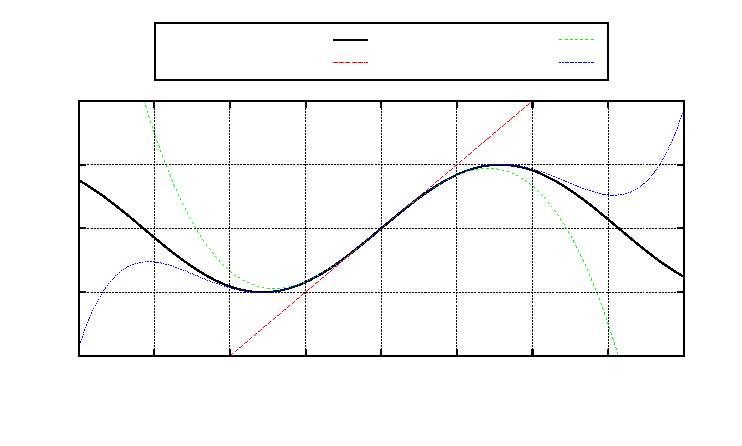
\includegraphics{taylor_sin}}%
    \gplfronttext
  \end{picture}%
\endgroup

\caption{}
\label{fig_taylor_sin}
\end{figure}

\end{document}